\documentclass{plt}

\usetikzlibrary{automata,positioning}
\usetikzlibrary{shadows}
\usetheme{metropolis}           % Use metropolis theme

%\DeclareSymbolFont{operator}{OT1}{put}{m}{n}
%\DeclareSymbolFont{letters}{OT1}{put}{m}{it}

\title{An Introduction to OCaml}
\author{Ronghui Gu}
\institute{Columbia University}
\date{Spring 2019}
\titlegraphic{
\includegraphics[width=0.2\textwidth]{caml-128x58.png}

\vspace{140pt}
{\tiny $^*$ Course website: \url{https://www.cs.columbia.edu/~rgu/courses/4115/spring2019}\vspace{-5pt}}\\
{\tiny $^{**}$ These slides are borrowed from Prof. Edwards.}
}

\begin{document}

\frame{\titlepage}


%\begin{frame}
%\vspace{25pt}
%
\includegraphics[width=1\textwidth]{happy-lunar-new-year-600x419.jpg}
%\thispagestyle{empty}
%\end{frame}

%\frame{\tableofcontents}

\begin{frame}{An Endorsement?}

A PLT student accurately summed up using OCaml:

\begin{quote}
Never have I spent \\ so much time \\ writing so little \\ that does so much.
\end{quote}

I think he was complaining, but I'm not sure.

Other students have said things like

\begin{quote}
It's hard to get it to compile, but once it compiles, it works.
\end{quote}

\end{frame}

\begin{frame}{Why OCaml?}

  \begin{itemize}
  \item \alert{It's Great for Compilers}

    I've written compilers in C++, Python, Java, and OCaml, and it's much
    easier in OCaml.

  \item \alert{It's Succinct}

    Would you prefer to write 10\,000 lines of code or 5\,000?
    
  \item \alert{Its Type System Catches Many Bugs}

    It catches missing cases, data structure misuse, certain off-by-one
    errors, etc.  Automatic garbage collection and lack of null pointers
    makes it safer than Java.
    
  \item \alert{Lots of Libraries and Support}
  
%    All sorts of data structures, I/O, OS interfaces, graphics, support for
%    compilers, etc.

  \item \alert{ Lots of Support}
    
%    Many websites, free online books and tutorials, code samples, etc.

\end{itemize}
\end{frame}


%\def\callout#1#2#3#4{\rnode{dest}{#3}\rput(#1,#2){\rnode{src}{\rmfamily\begin{tabular}{@{}l@{}}#4\end{tabular}}}\ncline[linecolor=red,nodesep=4pt]{src}{dest}}
\newcommand{\callout}[4]{%
  \begin{tikzpicture}[overlay]
    \draw node [anchor=south west,inner sep=0pt,color=white] at (0,0) (callout)
      {#3};
    \draw node at (#1,#2) (text)
       {\sffamily\begin{tabular}{@{}l@{}}#4\end{tabular}};
    \draw [color=red] (text) -- (callout);
  \end{tikzpicture}%
  #3%
}

\begin{frame}[fragile]{OCaml in One Slide}

\emph{Apply a function to each list element; save results in a list}

\vspace{3pc}
\hfill
\begin{minipage}{0.7\textwidth}
  \hspace{-5pc}
\small
  \ttfamily
\begin{tabbing}
\ \ \= \ \ \= \ \ \= \kill
\alert{\#} let \callout{-5pc}{3pc}{rec}{``Is recursive''} map \callout{3pc}{3pc}{f}{Passing a function} = function \\
\>\> [] -> [] \\
\> \callout{-6pc}{3pc}{|}{Case\\splitting} \callout{15pc}{3pc}{head\ ::\ tail}{Pattern\\Matching} -> \\
\>\>\> \callout{-7pc}{1pc}{let r}{Local name\\declaration} = f \callout{8pc}{2pc}{head}{Polymorphic} in \\
\>\>\> r \callout{-8pc}{-0.5pc}{::}{List support} \callout{-10pc}{-3pc}{map}{Recursion} f tail;; \\
\\
\alert{val map : \callout{12pc}{3pc}{('a -> 'b) -> 'a list -> 'b list}{Types inferred}} \\
\\
\alert{\#} map \callout{-7pc}{-2pc}{(function x -> x + 3)}{Anonymous\\functions} [1;5;9];; \\
\\
\alert{- : int list = [4; 8; 12]}
\end{tabbing}
\end{minipage}
\end{frame}

\part{The Basics}

\begin{frame}[fragile]{Hello World in OCaml: Interpret or Compile}

Create a ``hello.ml'' file:

\begin{ocaml}
print_endline "Hello World!"
\end{ocaml}

Run it with the interpreter:

\begin{interactive}
\$ \type{ocaml hello.ml}
Hello World!
\end{interactive}

\vspace{-15pt}
Run it with the \alert{bytecode} interpreter:
\begin{interactive}
\$ \type{ocamlc -o hello hello.ml}
\$ \type{ocamlrun hello}
Hello World!
\end{interactive}

\vspace{-15pt}
On most systems, the bytecode can be run directly:
\begin{interactive}
\$ \type{ocamlc -o hello hello.ml}
\$ \type{./hello}
Hello World!
\end{interactive}
\end{frame}

\begin{frame}[fragile]{Hello World in OCaml: Interpret or Compile}

Compile a native executable and run:

\begin{interactive}
\$ \type{ocamlopt -o hello hello.ml}
\$ \type{./hello}
Hello World!
\end{interactive}
%

Use ocamlbuild: built-in compilation rules for OCaml projects handle all the nasty cases;
automatic inference of dependencies, parallel compilation, etc.

\begin{interactive}
$ \type{ocamlbuild hello.native}
$ \type{./hello.native}
Hello World!
\end{interactive}

\end{frame}

\begin{frame}[fragile]{Hello World in OCaml: REPL}

  The interactive Read-Eval-Print Loop

\begin{interactive}
\$ \type{ocaml}
        OCaml version 4.02.3

# \type{print_endline "Hello World!";;}
Hello World!
- : unit = ()
# \type{#use "hello.ml";;}
Hello World!
- : unit = ()
# \type{#quit;;}
\$
\end{interactive}
%
Double semicolons \verb|;;| mean ``I'm done with this expression''

\#quit terminates the REPL

Other directives enable tracing, modify printing, and display types
and values. Use \alert{ledit ocaml} or \alert{utop} instead for better line
editing (history, etc.)

\end{frame}


\begin{frame}[fragile]{Comments}

  \begin{columns}
    \begin{column}[t]{0.5\textwidth}
OCaml
\begin{ocaml}
(* This is a multiline
   comment in OCaml *)

(* Comments
    (* like these *)
   do nest
*)

(* OCaml has no *)
(* single-line comments *)
\end{ocaml}
    \end{column}
    \begin{column}[t]{0.5\textwidth}
C/C++/Java
\begin{C}
/* This is a multiline
   comment in C */

/* C comments
     /* do not
   nest
 */

// C++/Java also has
// single-line comments
\end{C}
    \end{column}
  \end{columns}
\end{frame}

\begin{frame}[fragile]{Basic Types and Expressions}
\begin{minipage}{0.5\textwidth}
\begin{interactive}
# \type{42 + 17;;}
- : int = 59
\li
# \type{42.0 +. 18.3;;}
- : float = 60.3
\li
# \type{42 + \underline{60.3};;}
Error: This expression has type 
float but an expression was 
expected of type int
\li
# \type{42 + int_of_float 60.3;;}
- : int = 102
\li
# \type{true || (3 > 4) && not false;;}
- : bool = true
\li
# \type{"Hello " ^ "World!";;}
- : string = "Hello World!"
\li
# \type{String.contains "Hello" 'o';;}
- : bool = true
\li
# \type{();;}
- : unit = ()
\li
# \type{print_endline "Hello World!";;}
Hello World!
- : unit = ()
\end{interactive}
\end{minipage}\hfill%
\begin{minipage}{0.41\textwidth}
  \vspace{-20pt}
  \parskip=0.5\baselineskip
  \raggedright
  Integers (31-bit on 32-bit processors)

  Floating-point numbers
  
  Floating-point operators must be explicit (e.g., \texttt{+.})

  Only explicit conversions, promotions  (e.g., \texttt{int\_of\_float})

  Booleans

  Strings  
   
  The unit type is like ``void'' in C and Java
\end{minipage}
\end{frame}

\begin{frame}
  \frametitle{Standard Operators and Functions}

  \begin{tabular}{>{\ttfamily}ll}
\toprule
+ - * / mod & Integer arithmetic \\
\midrule
+. -. *. /. ** & Floating-point arithmetic \\
\midrule
ceil floor sqrt exp \\
log log10 cos sin & Floating-point functions \\
tan acos asin atan \\
\midrule
not \char`\&\char`\&{} \char`\|\char`\| & Boolean operators \\
\midrule
= \char`\<\char`\> & Structual comparison (polymorphic) \\
== != & Physical comparison (polymorphic) \\
\midrule
\char`\<{} \char`\>{} \char`\<= \char`\>= & Comparisons (polymorphic) \\
\midrule
  \end{tabular}

\end{frame}

\begin{frame}[fragile]{Structural vs. Physical Equality}

\begin{columns}
\begin{column}[t]{0.5\textwidth}      
\verb|==|, \verb|!=| Physical equality compares pointers

\begin{interactive}
# \type{1 == 3;;}
- : bool = false
\li
# \type{1 == 1;;}
- : bool = true
\li
# \type{1.5 == 1.5;;}
- : bool = false   \type{(* Huh? *)}
\li
# \type{let f = 1.5 in f == f;;}
- : bool = true
\li
# \type{'a' == 'a';;}
- : bool = true 
\li
# \type{"a" == "a";;}
- : bool = false   \type{(* Huh? *)}
\li
# \type{let a = "hello" in a == a;;}
- : bool = true
\end{interactive}
\end{column}%
\begin{column}[t]{0.5\textwidth}
\verb|=|, \verb|<>| Structural equality compares values
  
\begin{interactive}
# \type{1 = 3;;}
- : bool = false
\li
# \type{1 = 1;;}
- : bool = true
\li
# \type{1.5 = 1.5;;}
- : bool = true    
\li
# \type{let f = 1.5 in f = f;;}
- : bool = true
\li
# \type{'a' = 'a';;}
- : bool = true
\li
# \type{"a" = "a";;}
- : bool = true
\end{interactive}
Use structural equality to avoid headaches
\end{column}
\end{columns}

\end{frame}

\begin{frame}[fragile]{If-then-else}

  \begin{center}
  \textbf{\texttt{if}} \emph{expr}$_1$ \textbf{\texttt{then}}
  \emph{expr}$_2$ \textbf{\texttt{else}} \emph{expr}$_3$
  \end{center}

  If-then-else in OCaml is an expression.  The \emph{else} part is
  compulsory, \emph{expr}$_1$ must be Boolean, and the types of
  \emph{expr}$_2$ and \emph{expr}$_3$ must match.

\begin{interactive}
# \type{if 3 = 4 then 42 else 17;;}
- : int = 17
\li
# \type{if "a" = "a" then 42 else 17;;}
- : int = 42
\li
# \type{if true then 42 else \underline{"17"};;}
This expression has type string but is here used with type int
\end{interactive}

\end{frame}

\begin{frame}[fragile]{Naming Expressions with \emph{let}}

  \begin{tabular}{ll}
    \textbf{\texttt{let}} \emph{name} \textbf{\texttt{=}}
    \emph{expr}$_1$ \texttt{\textbf{in}} \emph{expr}$_2$ &
  Bind \emph{name} to \emph{expr}$_1$ in \emph{expr}$_2$ only
  \\
  \textbf{\texttt{let}} \emph{name} \textbf{\texttt{=}} \emph{expr} &
  Bind \emph{name} to \emph{expr} forever after  

  \end{tabular}
  
\begin{interactive}
# \type{let x = 38 in x + 4;;}
  - : int = 42
\li
# \type{let x = (let y = 2 in y + y) * 10 in x;;}
- : int = 40
\li
# \type{x + 4;;}
Unbound value x
\li
# \type{let x = 38;;}
val x : int = 38
\li
# \type{x + 4;;}
- : int = 42
\li
# \type{let x = (let y = 2\underline{)} * 10 in x;;}
Error: Syntax error: operator expected.
\li
# \type{let x = 10 in let y = x\underline{;;}}
Error: Syntax error
\end{interactive}

\end{frame}

\begin{frame}[fragile]{\emph{Let} is Not Assignment}

\emph{Let} can be used to bind a succession of values to a name.
This is not assignment: the value disappears in the end.

\begin{interactive}
# \type{let a = 4 in
  let a = a + 2 in
  let a = a * 2 in
  a;;}
- : int = 12

# \type{\underline{a};;}
Unbound value a
\end{interactive}

This looks like sequencing, but it is really data dependence.

\end{frame}

\begin{frame}[fragile]{\emph{Let} is Really Not Assignment}

OCaml picks up the values in effect where the function
is defined.
\alert{Global declarations are not like C's global variables.}

\begin{interactive}
# \type{let a = 5;;}
val a : int = 5
# \type{let adda x = x + a;;}
val adda : int -> int = <fun>

# \type{let a = 10;;}
val a : int = 10
# \type{adda 0;;}
- : int = 5        \alert{(* adda sees a = 5 *)}

# \type{let adda x = x + a;;}
val adda : int -> int = <fun>
# \type{adda 0;;}
- : int = 10       \alert{(* adda sees a = 10 *)}
\end{interactive}

\end{frame}

\part{Functions}


\begin{frame}[fragile]{Calling Functions}

  \begin{columns}
      \begin{column}[t]{0.5\textwidth}
C/C++/Java
\begin{C}
// This is C/C++/Java code
average (3, 4);
\end{C}
    \end{column}

    \begin{column}[t]{0.5\textwidth}
OCaml    
\begin{ocaml}
(* This is OCaml code*)
average 3.0 4.0
\end{ocaml}
    \end{column}

  \end{columns}

\vspace{20pt}
\alert{no} brackets and \alert{no} comma between the arguments
  
the syntax average (3.0, 4.0) is meaningful: call the function with ONE argument
has the type \alert{pair}
\end{frame}

\begin{frame}[fragile]{Defining Functions}

  \begin{columns}
      \begin{column}[t]{0.6\textwidth}
C/C++/Java

\begin{C}
double average (double a, double b)
{
  return (a + b) / 2;
}
\end{C}
    \end{column}
    \begin{column}[t]{0.3\textwidth}
OCaml

\begin{ocaml}
let average a b = 
  (a +. b) /. 2.0
\end{ocaml}
    \end{column}

  \end{columns}

type inference

no implicit casting
  
no \alert{return} keyword, the last expression becomes the result
\end{frame}

\begin{frame}[fragile]{Functions}

  A function is just another type whose value is an
  expression.

\begin{interactive}
# \type{fun x -> x * x;;}
- : int -> int = <fun>
# \type{(fun x -> x * x) 5;; (* function application *)}
- : int = 25
# \type{fun x -> (fun y -> x + y);;}
- : int -> int -> int = <fun>
# \type{fun x y -> x + y;;   (* shorthand *)}
- : int -> int -> int = <fun>
# \type{let plus = fun x y -> x + y;;}
val plus : int -> int -> int = <fun>
# \type{plus 2;;}
- : int -> int = <fun>
# \type{plus 2 3;;}
- : int = 5
# \type{let plus x y = x + y;; (* shorthand *)}
val plus : int -> int = <fun>
\end{interactive}
\end{frame}

\begin{frame}[fragile]{\emph{Let} is Like Function Application}

  \centerline{\textbf{\texttt{let}} \emph{name} \textbf{\texttt{=}}
    \emph{expr}$_1$ \texttt{\textbf{in}} \emph{expr}$_2$
  }

\vskip\baselineskip

\centerline{
  \texttt{(\textbf{fun}} \emph{name} \textbf{\texttt{->}}
  \emph{expr}$_2$\texttt{)} \emph{expr}$_1$
}

\vskip\baselineskip

Both mean ``\emph{expr}$_2$, with \emph{name} replaced by
\emph{expr}$_1$''

\begin{interactive}
# \type{let a = 3 in a + 2;;}
- : int = 5
  \li
# \type{(fun a -> a + 2) 3;;}
- : int = 5
\end{interactive}

Semantically equivalent; \texttt{let} is easier to read

\end{frame}

\begin{frame}[fragile]{Recursive Functions}

  \begin{columns}
    \begin{column}[t]{0.5\textwidth}
OCaml

\begin{ocaml}
let rec gcd a b =
  if a = b then
    a
  else if a > b then
    gcd (a - b) b
  else
    gcd a (b - a)
\end{ocaml}
    \end{column}
    \begin{column}[t]{0.5\textwidth}
C/C++/Java

\begin{C}
int gcd(int a, int b)
{
  while (a != b) {
    if (a > b)
      a -= b;
    else
      b -= a;
  }
  return a;
}
\end{C}
    \end{column}
  \end{columns}

\emph{let} \emph{rec} allows for recursion

Use recursion instead of loops
  
Tail recursion runs efficiently in OCaml
\end{frame}

\begin{frame}[fragile]{Recursive Functions}

By default, a name is not visible in its defining expression.

\begin{interactive}
# \type{let fac n = if n < 2 then 1 else n * \underline{fac} (n-1);;}
Unbound value fac
\end{interactive}
The \emph{rec} keyword makes the name visible.

\begin{interactive}
# \type{let rec fac n = if n < 2 then 1 else n * fac (n-1);;}
val fac : int -> int = <fun>
# \type{fac 5;;}
- : int = 120
\end{interactive}
The \emph{and} keyword allows for mutual recursion.

\begin{interactive}
# \type{let rec fac n = if n < 2 then 1 else n * fac1 n      
  and fac1 n = fac (n - 1);;}
val fac : int -> int = <fun>
val fac1 : int -> int = <fun>
# \type{fac 5;;}
- : int = 120
\end{interactive}

\end{frame}


\begin{frame}[fragile]{First-Class and Higher Order Functions}

  First-class functions are treated as values: name them, pass them as arguments,
  return them

\begin{interactive}
# \type{let plus5 x = x + 5;;}
val plus5 : int -> int = <fun>
# \type{let appadd f n= (f 42) + n;;}
val appadd : (int -> int) -> int -> int = <fun>
# \type{appadd plus5;;}
- : int -> int = <fun>
# \type{let appadd5 = appadd plus5;;}
val appadd5 : int -> int = <fun>
# \type{appadd5 17;;}
- : int = 64
\end{interactive}
Higher-order functions: functions that work on other functions

%\begin{interactive}
%# \type{let makeInc i = fun x -> x + i;;}
%val makeInc : int -> int -> int = <fun>
%# \type{let i5 = makeInc 5;;}
%val i5 : int -> int = <fun>
%# \type{i5 10;;}
%- : int = 15 
%\end{interactive}

\end{frame}

\part{Tuples, Lists, and Pattern Matching}

\begin{frame}[fragile]{Tuples}

Pairs or tuples of different types separated by commas.

Very useful lightweight data type, e.g., for function arguments.

\begin{interactive}
# \type{(18, "Adam");;}
- : int * string = (18, "Adam")
# \type{(18, "Adam", "CS");;}
- : int * string * string = (18, "Adam", "CS")
# \type{let p = (18, "Adam");;}
val p : int * string = (18, "Adam")
# \type{fst p;;}
- : int = 18
# \type{snd p;;}
- : string = "Adam"
# \type{let trip = (18, "Adam", "CS");;}
val trip : int * string * string = (18, "Adam", "CS")
# \type{let (age, _, dept) = trip in (age, dept);;}
- : int * string = (18, "CS")
\end{interactive}

\end{frame}



\begin{frame}[fragile]
  \frametitle{Records}

OCaml supports records much like C's \emph{structs}.

\begin{interactive}
# \type{type stu = \{age : int; name : string; dept : string \};;}
type stu = \{ age : int; name : string; dept : string; \}
# \type{let b0 = \{age = 18; name = "Adam"; dept = "CS" \};;}
val b0 : stu = \{age = 18; name = "Adam"; dept = "CS"\}
# \type{b0.name;;}
- : string = "Adam"
# \type{let b1 = \{ b0 with name = "Bob" \};;}
val b1 : stu = \{age = 18; name = "Bob"; dept = "CS"\}
# \type{let b2 = \{ b1 with age = 19; name = "Alice" \};;}
val b2 : stu = \{age = 19; name = "Alice"; dept = "CS"\}
\end{interactive}

\end{frame}


\begin{frame}[fragile]
  \frametitle{Lists}
\begin{ocaml}
(* Literals *)
[];;               (* The empty list *)
[1];;              (* A singleton list *)
[42; 16];;         (* A list of two integers *)
(* cons: Put something at the beginning *)
7 :: [5; 3];;      (* Gives [7; 5; 3] *)
[1; 2] :: [3; 4];; (* BAD: type error *)
(* concat: Append a list to the end of another *)
[1; 2] @ [3; 4];;  (* Gives [1; 2; 3; 4] *)
(* Extract first entry and remainder of a list *)
List.hd [42; 17; 28];; (* = 42 *)
List.tl [42; 17; 28];; (* = [17; 28] *)
\end{ocaml}

The elements of a list must all be the same type.

\verb|::| is very fast; \verb|@| is slower---$O(n)$

Pattern: create a list with cons, then use \emph{List.rev}.

\end{frame}

\begin{frame}[fragile]
  \frametitle{Some Useful List Functions}

Three great replacements for loops:

\verb|List.map f [a1; ... ;an] = [f a1; ... ;f an]|

Apply a function to each element of a list to produce another list.

%\vspace{10pt}
\begin{interactive}
# \type{List.map (fun a -> a + 10) [42; 17; 128];;}
- : int list = [52; 27; 138]
# \type{List.map string_of_int [42; 17; 128];;}
- : string list = ["42"; "17"; "128"]
\end{interactive}
\verb|List.fold_left f a [b1; ...;bn] =| \verb|f (...(f (f a b1) b2)...) bn|

Apply a function to a partial result and an element of the list to
produce the next partial result.

%\vspace{10pt}
\begin{interactive}
# \type{List.fold_left (fun sum e -> sum + e) 0 [42; 17; 128];;}
- : int = 187
\end{interactive}

\end{frame}

\begin{frame}[fragile]
  \frametitle{Some Useful List Functions}


\verb|List.iter f [a1; ...;an] = begin f a1; ... ; f an; () end|

Apply a function to each element; produce a unit result.


\begin{interactive}
# \type{List.iter print_int [42; 17; 128];;}
4217128- : unit = ()
# \type{List.iter (fun n -> print_int n; print_newline ())
   [42; 17; 128];;}
42
17
128
- : unit = ()
# \type{List.iter print_endline (List.map string_of_int [42; 17; 128]);;}
42
17
128
- : unit = ()
\end{interactive}
\verb|List.rev [a1; ...; an] = [an; ... ;a1]|

Reverse the order of the elements of a list.

\end{frame}

\begin{frame}[fragile]
  \frametitle{Example: Enumerating List Elements}

To transform a list and pass information between elements, use
\emph{List.fold\_left} with a tuple:

\begin{interactive}
# \type{let (l, _) = List.fold_left
    (fun (l, n) e -> ((e, n)::l, n+1)) ([], 0) [42; 17; 128]
  in List.rev l;;}
- : (int * int) list = [(42, 0); (17, 1); (128, 2)]
\end{interactive}
%Result accumulated in the \emph{(l, n)} tuple, \emph{List.rev}
%reverses the result (built backwards) in the end.  
Can do the same
with a recursive function.
%, but \emph{List.fold\_left} separates list
%traversal from modification:

\begin{interactive}
# \type{let rec enum n l =
   match l with
      | [] -> []
      | h :: t -> (h, n) :: enum (n + 1) t;;}
val enum : int -> 'a list -> ('a * int) list = <fun>
# \type{enum 0 [42; 17; 128];;}
- : (int * int) list = [(42, 0); (17, 1); (128, 2)]
\end{interactive}

\end{frame}

\begin{frame}[fragile]
  \frametitle{Example: Enumerating List Elements}

Using tail recursion:

\begin{interactive}
# \type{let rec enum rl n l =
   match l with
      | [] -> List.rev rl
      | h :: t -> enum ((h, n) :: rl) (n + 1) t;;}
val enum : ('a * int) list -> int -> 'a list -> ('a * int) list = <fun>
# \type{enum [] 0 [42; 17; 128];;}
- : (int * int) list = [(42, 0); (17, 1); (128, 2)]
\end{interactive}
%Result accumulated in the \emph{(l, n)} tuple, \emph{List.rev}
%reverses the result (built backwards) in the end.  
Using a \alert{helper} function:
%, but \emph{List.fold\_left} separates list
%traversal from modification:

\begin{interactive}
# \type{let enum l =
   let rec helper rl n l =
   match l with
      | [] -> List.rev rl
      | h :: t -> helper ((h, n) :: rl) (n + 1) t
   in helper [] 0 l;;}
val enum : int -> 'a list -> ('a * int) list = <fun>
# \type{enum [42; 17; 128];;}
- : (int * int) list = [(42, 0); (17, 1); (128, 2)]
\end{interactive}

\end{frame}

\begin{frame}[fragile]{Pattern Matching}

A powerful variety of multi-way branch that is adept at picking apart
data structures.  Unlike anything in C/C++/Java.

\begin{interactive}
# \type{let xor p = 
match p  with 
     | (false, false) -> false 
     | (false,  true) -> true 
     | (true, false) -> true 
     | (true,  true) -> false;;}
val xor : bool * bool -> bool = <fun>
# \type{xor (true, true);;}
- : bool = false
\end{interactive}
\end{frame}

\begin{frame}[fragile]{Pattern Matching}

A name in a pattern matches anything and is bound when the pattern
matches.  Each may appear only once per pattern.

\begin{interactive}
# \type{let xor p = 
match p with 
     | (false, x) -> x 
     | (true, x) -> not x;;}
val xor : bool * bool -> bool = <fun>
# \type{xor (true, true);;}
- : bool = false
\end{interactive}

\end{frame}

\begin{frame}[fragile]
  \frametitle{Case Coverage}

The compiler warns you when you miss a case or when one is redundant
(they are tested in order):

\begin{interactive}
# \type{let xor p = match p 
  with (false, x) -> x 
     | (x, true) -> not x;;}
Warning P: this pattern-matching is not exhaustive.
Here is an example of a value that is not matched:
(true, false)
val xor : bool * bool -> bool = <fun>

# \type{let xor p = match p 
  with (false, x) -> x 
     | (true,  x) -> not x 
     | \underline{(false, false)} -> false;;}
Warning U: this match case is unused.
val xor : bool * bool -> bool = <fun>
\end{interactive}

\end{frame}

\begin{frame}[fragile]
  \frametitle{Wildcards}

Underscore (\verb|_|) is a wildcard that will match anything, useful
as a default or when you just don't care.

\begin{interactive}
# \type{let xor p = match p 
  with (true, false) | (false, true) -> true 
     | _ -> false;;}
val xor : bool * bool -> bool = <fun>
# \type{xor (true, true);;}
- : bool = false
# \type{xor (true, false);;}
- : bool = true
# \type{let logand p = match p 
  with (false, _) -> false 
     | (true, x) -> x;;}
val logand : bool * bool -> bool = <fun>
# \type{logand (true, false);;}
- : bool = false
# \type{logand (true, true);;}
- : bool = true
\end{interactive}

\end{frame}

\begin{frame}[fragile]
  \frametitle{Pattern Matching with Lists}

\begin{interactive}
# \type{let length = function (* let length = fun p -> match p with *)
  | [] -> "empty" 
  | [_] -> "singleton" 
  | [_; _] -> "pair" 
  | [_; _; _] -> "triplet" 
  | hd :: tl -> "many";;}
val length : 'a list -> string = <fun>

# \type{length [];;}
- : string = "empty"

# \type{length [1; 2];;}
- : string = "pair"

# \type{length ["foo"; "bar"; "baz"];;}
- : string = "triplet"

# \type{length [1; 2; 3; 4];;}
- : string = "many"
\end{interactive}

\end{frame}

\begin{frame}[fragile]{Pattern Matching with \emph{when} and \emph{as}}

The \emph{when} keyword lets you add a guard expression:

\begin{interactive}
# \type{let tall = function 
  | (h, s) when h > 180 -> s ^ " is tall" 
  | (_, s) -> s ^ " is short";;} 
val tall : int * string -> string = <fun>
# \type{List.map  tall [(183, "Stephen"); (150, "Nina")];;}
- : string list = ["Stephen is tall"; "Nina is short"]
\end{interactive}

The \emph{as} keyword lets you name parts of a matched structure:

\begin{interactive}
# \type{match ([3,9], 4) with  
  | (3::_ as xx, 4) -> xx 
  | _ -> [];;}
- : int * int = (3, 9)
\end{interactive}

\end{frame}

\begin{frame}[fragile]
  \frametitle{Application: Length of a list}

\begin{ocaml}
let rec length l =
  if l = [] then 0 else 1 + length (List.tl l);;
\end{ocaml}

Correct, but not very elegant.  With pattern matching,

\begin{ocaml}
let rec length = function
 |  []    -> 0
 | _::tl -> 1 + length tl;;
\end{ocaml}

Elegant, but inefficient because it is not tail-recursive (needs
$O(n)$ stack space).  Common trick: use an argument as an accumulator.

\begin{ocaml}
let length l =
  let rec helper len = function
    |  []    -> len
    | _::tl -> helper (len + 1) tl
  in helper 0 l
\end{ocaml}

This is the code for the List.length standard library function.

\end{frame}

\begin{frame}[fragile]
  \frametitle{OCaml Can Compile This Efficiently}

% ocamlopt -S -c length.ml

  \begin{columns}
    \begin{column}[t]{0.6\textwidth}

OCaml source code

\medskip

\begin{ocaml}
let length list =
  let rec helper len = function
      []    -> len
    | _::tl -> helper (len + 1) tl
  in helper 0 list
\end{ocaml}

\begin{itemize}
\item Arguments in registers
\item Pattern matching reduced to a conditional branch
\item Tail recursion implemented with jumps
\item LSB of an integer always~1
\end{itemize}

    \end{column}
    \begin{column}[t]{0.4\textwidth}
ocamlopt generates this x86 assembly pseudocode 

\medskip

\begin{interactive}
\color{black}camlLength__helper:
.L101:
  cmpl  $1, %ebx      \alert{# empty?}
  je    .L100
  movl  4(%ebx), %ebx \alert{# get tail}
  addl  $2, %eax      \alert{# len++}
  jmp   .L101
.L100:
  ret

camlLength__length:
  movl  %eax, %ebx
  movl  $1, %eax     \alert{# len = 0}
  jmp   camlLength__helper
\end{interactive}    
    \end{column}
  \end{columns}

\end{frame}

\part{User-Defined Types}

\begin{frame}[fragile]
  \frametitle{Type Declarations}

A new type name is defined globally.  Unlike \emph{let}, \emph{type}
is recursive by default, so the name being defined may appear in the
\emph{typedef}.

  \begin{center}
    \textbf{\texttt{type}} \emph{name} \textbf{\texttt{=}} \emph{typedef}
  \end{center}

Mutually-recursive types can be defined with \emph{and}.

\begin{center}
\begin{tabular}{l@{\;}l}
\textbf{\texttt{type}} & \emph{name}$_1$ \textbf{\texttt{=}}
\emph{typedef}$_1$ \\
\textbf{\texttt{and}} & \emph{name}$_2$ \textbf{\texttt{=}}
\emph{typedef}$_2$ \\
& \multicolumn{1}{c}{$\vdots$} \\
\textbf{\texttt{and}} & \emph{name}$_n$ \textbf{\texttt{=}}
\emph{typedef}$_n$ \\
\end{tabular}
\end{center}

\end{frame}

\begin{frame}[fragile]
  \frametitle{Records}

OCaml supports records much like C's \emph{structs}.

\begin{interactive}
# \type{type base = \{ x : int; y : int; name : string \};;}
type base = \{ x : int; y : int; name : string; \}
# \type{let b0 = \{ x = 0; y = 0; name = "home" \};;}
val b0 : base = \{x = 0; y = 0; name = "home"\}
# \type{let b1 = \{ b0 with x = 90; name = "first" \};;}
val b1 : base = \{x = 90; y = 0; name = "first"\}
# \type{let b2 = \{ b1 with y = 90; name = "second" \};;}
val b2 : base = \{x = 90; y = 90; name = "second"\}
# \type{b0.name;;}
- : string = "home"
# \type{let dist b1 b2 = 
    let hyp x y = sqrt (float_of_int (x*x + y*y)) in 
    hyp (b1.x - b2.x) (b1.y - b2.y);;}
val dist : base -> base -> float = <fun>
# \type{dist b0 b1;;}
- : float = 90.
# \type{dist b0 b2;;}
- : float = 127.279220613578559
\end{interactive}

\end{frame}

\begin{frame}[fragile]
  \frametitle{Algebraic Types/Tagged Unions/Sum-Product Types}

Vaguely like C's \emph{union}s, \emph{enum}s, or a class hierarchy:
objects that can be one of a set of types.  In compilers, great for
trees and instructions.

\begin{interactive}
# \type{type seasons = Winter | Spring | Summer | Fall;;}
type seasons = Winter | Spring | Summer | Fall
# \type{let weather = function 
  | Winter -> "Too Cold" 
  | Spring -> "Too Wet" 
  | Summer -> "Too Hot" 
  | Fall -> "Too Short";;}
val weather : seasons -> string = <fun>

# \type{weather Spring;;}
- : string = "Too Wet"

# \type{let year = [Winter; Spring; Summer; Fall] in 
  List.map weather year;;}
- : string list = ["Too Cold"; "Too Wet"; "Too Hot"; "Too Short"]
\end{interactive}

\end{frame}

\begin{frame}[fragile]
  \frametitle{Simple Syntax Trees and an Interpreter}

\begin{interactive}
# \type{type expr = 
    Lit of int 
  | Plus of expr * expr 
  | Minus of expr * expr 
  | Times of expr * expr;;}
type expr =
    Lit of int
  | Plus of expr * expr
  | Minus of expr * expr
  | Times of expr * expr
# \type{let rec eval = function
    Lit(x) -> x 
  | Plus(e1, e2) -> (eval e1) + (eval e2) 
  | Minus(e1, e2) -> (eval e1) - (eval e2) 
  | Times(e1, e2) -> (eval e1) * (eval e2);;}
val eval : expr -> int = <fun>
# \type{eval (Lit(42));;}
- : int = 42
# \type{eval (Plus(Lit(17), Lit(25)));;}
- : int = 42
\end{interactive}
\end{frame}

\begin{frame}[fragile]
  \frametitle{Algebraic Type Rules}

Each tag name must begin with a capital letter

\medskip

\begin{interactive}
# \type{let bad1 = left \underline{|} right;;}
Syntax error
\end{interactive}

\medskip

Tag names must be globally unique (required for type inference)

\medskip

\begin{interactive}
# \type{type weekend = Sat | Sun;;}
type weekend = Sat | Sun
# \type{type days = Sun | Mon | Tue;;}
type days = Sun | Mon | Tue
# \type{function Sat -> "sat" | \underline{Sun} -> "sun";;}
This pattern matches values of type days
but is here used to match values of type weekend
\end{interactive}

\end{frame}

\begin{frame}[fragile]
  \frametitle{Algebraic Types and Pattern Matching}

The compiler warns about missing cases:

\begin{interactive}
# \type{type expr = 
    Lit of int 
  | Plus of expr * expr 
  | Minus of expr * expr 
  | Times of expr * expr;;}
type expr =
    Lit of int
  | Plus of expr * expr
  | Minus of expr * expr
  | Times of expr * expr
# \type{let rec eval = \underline{function}
\underline{    Lit(x) -> x}
\underline{  | Plus(e1, e2) -> (eval e1) + (eval e2)}
\underline{  | Minus(e1, e2) -> (eval e1) - (eval e2)};;}
Warning P: this pattern-matching is not exhaustive.
Here is an example of a value that is not matched:
Times (_, _)
val eval : expr -> int = <fun>
\end{interactive}

\end{frame}

\begin{frame}[fragile]
  \frametitle{The \emph{Option} Type: A Safe Null Pointer}

Part of the always-loaded core library:

\begin{center}
\texttt{type 'a option = None | Some of 'a}
\end{center}

This is a polymorphic algebraic type: \texttt{'a} is any type.
\emph{None} is like a null pointer; \emph{Some} is a non-null pointer.
The compiler requires \emph{None} to be handled explicitly.

\begin{interactive}
# \type{let rec sum = function 
    []          -> 0                            (* base case *)
  | None::tl    -> sum tl  (* handle the "null pointer" case *)
  | Some(x)::tl -> x + sum tl;;               (* normal case *)}
val sum : int option list -> int = <fun>

# \type{sum [None; Some(5); None; Some(37)];;}
- : int = 42
\end{interactive}

\end{frame}

\begin{frame}
  \frametitle{Algebraic Types vs. Classes and Enums}

\begin{tabular}{llll}
\toprule
& \textbf{Algebraic Types} & \textbf{Classes} & \textbf{Enums} \\
\midrule
\textbf{Choice of Types} & fixed & extensible & fixed \\
\textbf{Operations} & extensible & fixed & extensible \\[5pt]
\textbf{Fields} & ordered & named & none \\
\textbf{Hidden fields} & none & supported & none \\
\textbf{Recursive} & yes & yes & no \\
\textbf{Inheritance} & none & supported & none \\
\textbf{Case splitting} & simple & costly & simple \\
\bottomrule
\end{tabular}

\medskip

An algebraic type is best when the set of types rarely change but you
often want to add additional functions.  Classes are good in exactly
the opposite case.

\end{frame}

\part{Modules and Compilation}

\begin{frame}[fragile]{Modules}

Each source file is a module and everything is public.

\vspace{1pc}

\begin{columns}
  \begin{column}[t]{0.5\textwidth}
foo.ml
\medskip
\begin{ocaml}
(* Module Foo *)

type t = { x : int ; y : int }
let sum c = c.x + c.y
\end{ocaml}

\vspace{1pc}

To compile and run these,

\medskip

\begin{interactive}
$ \type{ocamlc -c foo.ml}
  (creates foo.cmi foo.cmo)
$ \type{ocamlc -c bar.ml}
  (creates bar.cmi bar.cmo)
$ \type{ocamlc -o ex foo.cmo bar.cmo}
$ \type{./ex}
333
\end{interactive}
% $

  \end{column}
  \begin{column}[t]{0.5\textwidth}
bar.ml
\medskip
\begin{ocaml}
(* The dot notation *)

let v = { Foo.x = 1 ;
          Foo.y = 2 };;
print_int (Foo.sum v)

(* Create a short name *)

module F = Foo;;
print_int (F.sum v)

(* Import every name from
   a module with "open" *)

open Foo;;
print_int (sum v)
\end{ocaml}
  \end{column}
\end{columns}

\end{frame}

\begin{frame}[fragile]
  \frametitle{Separating Interface and Implementation}

\begin{columns}
  \begin{column}[t]{0.5\textwidth}
stack.mli
\medskip
\begin{ocaml}
type 'a t

exception Empty

val create : unit -> 'a t
val push : 'a -> 'a t -> unit
val pop : 'a t -> 'a
val top : 'a t -> 'a
val clear : 'a t -> unit
val copy : 'a t -> 'a t
val is_empty : 'a t -> bool
val length : 'a t -> int
val iter : ('a -> unit) ->
                 'a t -> unit
\end{ocaml}
  \end{column}
  \begin{column}[t]{0.5\textwidth}
stack.ml
\medskip
\begin{ocaml}
type 'a t =
   { mutable c : 'a list }
exception Empty
let create () = { c = [] }
let clear s = s.c <- []
let copy s = { c = s.c }
let push x s = s.c <- x :: s.c
let pop s =
  match s.c with
    hd::tl -> s.c <- tl; hd
  | []     -> raise Empty
let top s =
  match s.c with
    hd::_ -> hd
  | []    -> raise Empty
let is_empty s = (s.c = [])
let length s = List.length s.c
let iter f s = List.iter f s.c
\end{ocaml}
  \end{column}
\end{columns}

\end{frame}


\part{Exceptions}

\begin{frame}[fragile]{Exceptions}

\begin{interactive}
# \type{5 / 0;;}
Exception: Division_by_zero.

# \type{try 
    5 / 0 
  with Division_by_zero -> 42;;}
- : int = 42

# \type{exception My_exception;;}
exception My_exception
# \type{try 
    if true then
       raise My_exception
    else 0
  with My_exception -> 42;;}
- : int = 42
\end{interactive}

\end{frame}

\begin{frame}[fragile]{Exceptions}

\begin{interactive}
# \type{exception Foo of string;;}
exception Foo of string
# \type{exception Bar of int * string;;}
exception Bar of int * string

# \type{let ex b = 
  try 
    if b then    
      raise (Foo("hello"))
    else 
      raise (Bar(42, " answer"))
  with Foo(s) -> "Foo: " ^ s
  | Bar(n, s) -> "Bar: " ^ string_of_int n ^ s;;}
val ex : bool -> unit = <fun>

# \type{ex true;;}
- : string = "Foo: hello"
# \type{ex false;;}
- : string = "Bar: 42 answer"
\end{interactive}

\end{frame}

\part{Standard Library Modules}

\begin{frame}[fragile]{Maps}

\begin{scriptsize}
Balanced trees for implementing dictionaries.  Ask for a map with a
specific kind of key; values are polymorphic.

\begin{interactive}
# \type{module StringMap = Map.Make(String);;}
module StringMap :
  sig
    type key = String.t
    type 'a t = 'a Map.Make(String).t
    val empty : 'a t
    val is_empty : 'a t -> bool
    val add : key -> 'a -> 'a t -> 'a t
    val find : key -> 'a t -> 'a
    val remove : key -> 'a t -> 'a t
    val mem : key -> 'a t -> bool
    val iter : (key -> 'a -> unit) -> 'a t -> unit
    val map : ('a -> 'b) -> 'a t -> 'b t
    val mapi : (key -> 'a -> 'b) -> 'a t -> 'b t
    val fold : (key -> 'a -> 'b -> 'b) -> 'a t -> 'b -> 'b
    val compare : ('a -> 'a -> int) -> 'a t -> 'a t -> int
    val equal : ('a -> 'a -> bool) -> 'a t -> 'a t -> bool
  end
\end{interactive}
\end{scriptsize}

\end{frame}

\begin{frame}[fragile]
  \frametitle{Maps}

\begin{interactive}
# \type{let mymap = StringMap.empty;;          (* Create empty map *)}
val mymap : 'a StringMap.t = <abstr>
# \type{let mymap = StringMap.add "Douglas" 42 mymap;; (* Add pair *)}
val mymap : int StringMap.t = <abstr>
# \type{StringMap.mem "foo" mymap;;             (* Is "foo" there? *)}
- : bool = false
# \type{StringMap.mem "Douglas" mymap;;     (* Is "Douglas" there? *)}
- : bool = true
# \type{StringMap.find "Douglas" mymap;;              (* Get value *)}
- : int = 42
# \type{let mymap = StringMap.add "Adams" 17 mymap;;}
val mymap : int StringMap.t = <abstr>
# \type{StringMap.find "Adams" mymap;;}
- : int = 17
# \type{StringMap.find "Douglas" mymap;;}
- : int = 42
# \type{StringMap.find "Slarti" mymap;;}
Exception: Not_found.
\end{interactive}
\end{frame}

\begin{frame}[fragile]
  \frametitle{Maps}

\begin{itemize}
\item Fully functional: \emph{Map.add} takes a key, a value, and a map
  and returns a new map that also includes the given key/value pair.

\item Needs a totally ordered key type. \emph{Pervasives.compare}
  usually does the job (returns $-1$, $0$, or $1$); you may
  supply your own.

\begin{minipage}{0.7\textwidth}
\begin{ocaml}
module StringMap = Map.Make(struct
  type t = string
  let compare x y = Pervasives.compare x y
end)
\end{ocaml}
\end{minipage}

\item Uses balanced trees, so searching and insertion is $O(\log n)$.

\end{itemize}

\end{frame}

\if 0
\begin{frame}[fragile]
  \frametitle{Imperative Features}

\begin{itemize}

\item The \emph{unit} type is something like \emph{void} in C/C++/Java.

\emph{Unit} is the return value of a function that does not produce a result.

\item The semicolon denotes sequencing.

\emph{expr}$_1$ \texttt{;}
  \emph{expr}$_2$ means evaluate \emph{expr}$_1$, which should be of
  \emph{unit} type, then evaluate \emph{expr}$_2$.

\item I/O operations return the \emph{unit} type.

\item Some data structures, e.g., arrays, are \emph{mutable}.

Mutable data can be modified by imperative-style code.  It is really
not functional, but sometimes more convenient
\end{itemize}

\end{frame}

\fi


\begin{frame}[fragile]
  \frametitle{Imperative Features}

\begin{interactive}
# \type{\underline{0} ; 42;;                           (* ";" means sequencing *)}
Warning S: this expression should have type unit.
- : int = 42
# \type{ignore 0 ; 42;;        (* ignore is a function: 'a -> unit *)}
- : int = 42
# \type{() ; 42;;           (* () is the literal for the unit type *)}
- : int = 42
# \type{print_endline "Hello World!";;    (* Print; result is unit *)}
Hello World!
- : unit = ()
# \type{print_string "Hello " ; print_endline "World!";;}
Hello World!
- : unit = ()
# \type{print_int 42 ; print_newline ();;}
42
- : unit = ()
# \type{print_endline ("Hello " ^ string_of_int 42 ^ " world!");;}
Hello 42 world!
- : unit = ()
\end{interactive}

\end{frame}

\begin{frame}[fragile]{Hash Tables}

\begin{interactive}
# \type{module StringHash = Hashtbl.Make(struct 
    type t = string                         (* type of keys *)
    let equal x y = x = y      (* use structural comparison *)
    let hash = Hashtbl.hash        (* generic hash function *)
  end);;}
module StringHash :
  sig
    type key = string
    type 'a t
    val create : int -> 'a t
    val clear : 'a t -> unit
    val copy : 'a t -> 'a t
    val add : 'a t -> key -> 'a -> unit
    val remove : 'a t -> key -> unit
    val find : 'a t -> key -> 'a
    val find_all : 'a t -> key -> 'a list
    val replace : 'a t -> key -> 'a -> unit
    val mem : 'a t -> key -> bool
    val iter : (key -> 'a -> unit) -> 'a t -> unit
    val fold : (key -> 'a -> 'b -> 'b) -> 'a t -> 'b -> 'b
    val length : 'a t -> int
  end
\end{interactive}

\end{frame}

\begin{frame}[fragile]
  \frametitle{Hash Tables}

\begin{interactive}
# \type{let hash = StringHash.create 17;;  (* initial size estimate *)}
val hash : '_a StringHash.t = <abstr>
# \type{StringHash.add hash "Douglas" 42;; (* modify the hash table *)}
- : unit = ()
# \type{StringHash.mem hash "foo";;              (* is "foo" there? *)}
- : bool = false
# \type{StringHash.mem hash "Douglas";;      (* is "Douglas" there? *)}
- : bool = true
# \type{StringHash.find hash "Douglas";;               (* Get value *)}
- : int = 42
# \type{StringHash.add hash "Adams" 17;;   (* Add another key/value *)}
- : unit = ()
# \type{StringHash.find hash "Adams";;}
- : int = 17
# \type{StringHash.find hash "Douglas";;}
- : int = 42
# \type{StringHash.find hash "Slarti";;}
Exception: Not_found.
\end{interactive}

\end{frame}

\begin{frame}[fragile]
  \frametitle{Arrays}

\begin{interactive}
# \type{let a = [| 42; 17; 19 |];;                (* Array literal *)}
val a : int array = [|42; 17; 19|]
# \type{let aa = Array.make 5 0;;              (* Fill a new array *)}
val aa : int array = [|0; 0; 0; 0; 0|]
# \type{a.(0);;                                   (* Random access *)}
- : int = 42
# \type{a.(2);;}
- : int = 19
# \type{a.(3);;}
Exception: Invalid_argument "index out of bounds".
# \type{a.(2) <- 20;;                       (* Arrays are mutable! *)}
- : unit = ()
# \type{a;;}
- : int array = [|42; 17; 20|]
# \type{let l = [24; 32; 17];;}
val l : int list = [24; 32; 17]
# \type{let b = Array.of_list l;;             (* Array from a list *)}
val b : int array = [|24; 32; 17|]
# \type{let c = Array.append a b;;                (* Concatenation *)}
val c : int array = [|42; 17; 20; 24; 32; 17|]
\end{interactive}

\end{frame}

\begin{frame}
  \frametitle{Arrays vs. Lists}

  \begin{center}
    \begin{tabular}{lll}
\toprule
& \textbf{Arrays} & \textbf{Lists} \\
\midrule
\textbf{Random access} & $O(1)$ & $O(n)$ \\
\textbf{Appending} & $O(n)$ & $O(1)$ \\
\textbf{Mutable} & Yes & No \\
\bottomrule
    \end{tabular}
  \end{center}

\medskip

Useful pattern: first collect data of unknown length in a list then
convert it to an array with \emph{Array.of\_list} for random queries.

\end{frame}


\part{A Complete Interpreter in Three Slides}
%\frame{\partpage}

\begin{frame}[fragile]
  \frametitle{The Scanner and AST}
scanner.mll

%\vspace{4pt}

\begin{ocamllex}
{ open Parser }

rule token =
  parse [' ' '\t' '\r' '\n'] { token lexbuf }
      | '+'                  { PLUS }
      | '-'                  { MINUS }
      | '*'                  { TIMES }
      | '/'                  { DIVIDE }
      | ['0'-'9']+ as lit    { LITERAL(int_of_string lit) }
      | eof                  { EOF }
\end{ocamllex}

%\vspace{1pc}

ast.mli

%\vspace{4pt}

\begin{ocaml}
type operator = Add | Sub | Mul | Div

type expr =
    Binop of expr * operator * expr
  | Lit of int
\end{ocaml}

\end{frame}

\begin{frame}[fragile]
  \frametitle{The Parser}

parser.mly

\vspace{4pt}

\begin{ocamlyacc}
%{ open Ast %}

%token PLUS MINUS TIMES DIVIDE EOF
%token <int> LITERAL

%left PLUS MINUS
%left TIMES DIVIDE

%start expr
%type <Ast.expr> expr

expr:
  expr PLUS   expr  { Binop($1, Add, $3) }
| expr MINUS  expr  { Binop($1, Sub, $3) }
| expr TIMES  expr  { Binop($1, Mul, $3) }
| expr DIVIDE expr  { Binop($1, Div, $3) }
| LITERAL           { Lit($1) }
\end{ocamlyacc}
% $
\end{frame}

\begin{frame}[fragile]
  \frametitle{The Interpeter}

calc.ml

\vspace{4pt}

\begin{ocaml}
open Ast

let rec eval = function 
    Lit(x) -> x
  | Binop(e1, op, e2) ->
      let v1 = eval e1 and v2 = eval e2 in
      match op with
        Add -> v1 + v2
      | Sub -> v1 - v2
      | Mul -> v1 * v2
      | Div -> v1 / v2

let _ =
  let lexbuf = Lexing.from_channel stdin in
  let expr = Parser.expr Scanner.token lexbuf in
  let result = eval expr in
  print_endline (string_of_int result)
\end{ocaml}

\end{frame}

\begin{frame}[fragile]{Compiling the Interpreter}

\begin{semiverbatim}
$ \alert{ocamllex scanner.mll # create scanner.ml}
8 states, 267 transitions, table size 1116 bytes
$ \alert{ocamlyacc parser.mly # create parser.ml and parser.mli}
$ \alert{ocamlc -c ast.mli    # compile AST types}
$ \alert{ocamlc -c parser.mli # compile parser types}
$ \alert{ocamlc -c scanner.ml # compile the scanner}
$ \alert{ocamlc -c parser.ml  # compile the parser}
$ \alert{ocamlc -c calc.ml    # compile the interpreter}
$ \alert{ocamlc -o calc parser.cmo scanner.cmo calc.cmo}
$ \alert{./calc}
\alert{2 * 3 + 4 * 5}
26
$
\end{semiverbatim}

\end{frame}

\begin{frame}[fragile]{Compiling with \emph{ocamlbuild}}

\begin{semiverbatim}
$ \alert{ls}
ast.mli  calc.ml  parser.mly  scanner.mll
$ \alert{ocamlbuild calc.native   # Build everything}
Finished, 15 targets (0 cached) in 00:00:00.
$ \alert{ls}
ast.mli _build calc.ml calc.native parser.mly scanner.mll
$ \alert{./calc.native}
\alert{2 * 3 + 4 * 5}
\alert{\emph{Ctrl-D}}
26
 \alert{ocamlbuild -clean # Remove _build and all .native}
\end{semiverbatim}
  
\end{frame}

\part{Directed Graphs}
\newcommand{\graph}{
  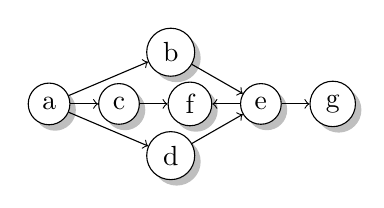
\begin{tikzpicture}[node distance=10pt,
      every node/.style={state, inner sep=3pt,minimum size=10pt,drop shadow,fill=white}]
    \node (a) {a};
    \node (c) [right=of a] {c};
    \node (f) [right=of c] {f};
    \node (b) [above right=of c] {b};
    \node (d) [below right=of c] {d};
    \node (e) [right=of f] {e};
    \node (g) [right=of e] {g};
    \path[->] (a) edge (c)
                  edge (b)
                  edge (d)
              (c) edge (f)
              (b) edge (e)
              (d) edge (e)
              (e) edge (f)
                  edge (g);
  \end{tikzpicture}
}

\begin{frame}[fragile]
  \frametitle{Application: Directed Graphs}

\begin{minipage}{0.6\textwidth}
\begin{ocaml}
let edges = [
  ("a", "b"); ("a", "c");
  ("a", "d"); ("b", "e");
  ("c", "f"); ("d", "e");
  ("e", "f"); ("e", "g") ]

let rec successors n = function
    []              -> []
  | (s, t) :: edges ->
      if s = n then
         t :: successors n edges
      else
         successors n edges
\end{ocaml}
\end{minipage}%
\begin{minipage}{0.4\textwidth}
  \graph
\end{minipage}

\begin{interactive}
# \type{successors "a" edges;;}
- : string list = ["b"; "c"; "d"]

# \type{successors "b" edges;;}
- : string list = ["e"]
\end{interactive}

\end{frame}

\begin{frame}[fragile]
  \frametitle{More Functional Successors}

\begin{ocaml}
let rec successors n = function
    []              -> []
  | (s, t) :: edges ->
      if s = n then
         t :: successors n edges
      else
         successors n edges
\end{ocaml}

\vspace{-5pt}
Our first example is imperative: performs ``search a list,'' which is more
precisely expressed using the library function \texttt{List.filter}:

\begin{ocaml}
let successors n edges = 
    let matching (s,_) = s = n in
    List.map snd (List.filter matching edges)
\end{ocaml}
\vspace{-5pt}

This uses the built-in \texttt{snd} function, which is defined as
\begin{ocaml}
let snd (_,x) = x
\end{ocaml}

\end{frame}

\begin{frame}[fragile]
  \frametitle{Depth-First Search}

\graph

\begin{ocaml}
let rec dfs edges visited = function
  []       -> List.rev visited
| n::nodes ->
  if List.mem n visited then
    dfs edges visited nodes
  else
    dfs edges (n::visited) ((successors n edges) @ nodes)
\end{ocaml}

\begin{interactive}
# \type{dfs edges [] ["a"];;}
- : string list = ["a"; "b"; "e"; "f"; "g"; "c"; "d"]
# \type{dfs edges [] ["e"];;}
- : string list = ["e"; "f"; "g"]
# \type{dfs edges [] ["d"];;}
- : string list = ["d"; "e"; "f"; "g"]
\end{interactive}

\end{frame}

\begin{frame}[fragile]
  \frametitle{Topological Sort}

\graph
Remember the visitor at the end.

\begin{ocaml}
let rec tsort edges visited = function
  []       -> visited
| n::nodes ->
  let visited' = if List.mem n visited then visited
                 else n :: tsort edges visited (successors n edges)
  in tsort edges visited' nodes;;
\end{ocaml}

\begin{interactive}
# \type{tsort edges [] ["a"];;}
- : string list = ["a"; "d"; "c"; "b"; "e"; "g"; "f"]
# \type{let cycle = [ ("a", "b"); ("b", "c"); ("c", "a") ];;}
val cycle : (string * string) list = [("a", "b"); ...]
# \type{tsort cycle [] ["a"];;}
Stack overflow during evaluation (looping recursion?).
\end{interactive}

\end{frame}

\begin{frame}[fragile]
  \frametitle{Better Topological Sort}

\begin{ocaml}
exception Cyclic of string
let tsort edges seed =
  let rec sort path visited = function
     []       -> visited
  |  n::nodes ->
     if List.mem n path then raise (Cyclic n) else
     let v' = if List.mem n visited then visited else
              n :: sort (n::path) visited (successors n edges)
     in sort path v' nodes
  in
  sort [] [] [seed]
\end{ocaml}

\begin{interactive}
# \type{tsort edges "a";;}
- : string list = ["a"; "d"; "c"; "b"; "e"; "g"; "f"]
# \type{tsort edges "d";;}
- : string list = ["d"; "e"; "g"; "f"]
# \type{tsort cycle "a";;}
Exception: Cyclic "a".
\end{interactive}

\end{frame}


\begin{frame}[fragile]
  \frametitle{Depth-First Search Revisited}

Previous version

\begin{ocaml}
let rec dfs edges visited = function
  []       -> List.rev visited
| n::nodes ->
  if List.mem n visited then
    dfs edges visited nodes
  else
    dfs edges (n::visited) ((successors n edges) @ nodes)
\end{ocaml}

was not very efficient, but good enough for small graphs.

Would like faster \emph{visited} test and \emph{successors} query.

\end{frame}

\begin{frame}[fragile]
  \frametitle{Depth-First Search Revisited}

Second version:

\begin{itemize}
\item use a Map to hold a list of successors for each node
\item use a Set (valueless Map) to remember of visited nodes
\end{itemize}

\begin{ocaml}
module StringMap = Map.Make(String)
module StringSet = Set.Make(String)
\end{ocaml}

\end{frame}

\lstset{
  language=[Objective]caml,
  basicstyle={\fontsize{7}{7}\selectfont\ttfamily\spaceskip=2pt},
} 


\begin{frame}[fragile]
  \frametitle{Depth-First Search Revisited}


\begin{ocaml}
let top_sort_map edges =
  (* Create an empty successor list for each node *)
  let succs = List.fold_left
      (fun map (s,d) ->
        StringMap.add d [] (StringMap.add s [] map)
      ) StringMap.empty edges
  in (* Build the successor list for each source node *)
  let succs = List.fold_left
      (fun succs (s, d) ->
        let ss = StringMap.find s succs
        in StringMap.add s (d::ss) succs) succs edges
  in 
  (* Visit recursively, storing each node after visiting successors*)
  let rec visit (order, visited) n =
    if StringSet.mem n visited then
      (order, visited)
    else  let (order, visited) = List.fold_left
              visit (order, StringSet.add n visited)
              (StringMap.find n succs)
          in (n::order, visited)
  in (* Visit the source of each edge *)
  fst (List.fold_left visit ([], StringSet.empty) 
                            (List.map fst edges))
\end{ocaml}

\end{frame}


\begin{frame}
  \frametitle{DFS with Arrays}

Second version used a lot of \emph{mem}, \emph{find}, and \emph{add}
calls on the string map, each $O(\log n)$.  Can we do better?

Solution: use arrays to hold adjacency lists and track visiting
information.

Basic idea: number the nodes, build adjacency lists with numbers, use
an array for tracking visits, then transform back to list of node names.

\end{frame}

\begin{frame}[fragile]{DFS with Arrays 1/2}

\begin{ocaml}
let top_sort_array edges =
  (* Assign a number to each node *)
  let map, nodecount =
    List.fold_left
      (fun nodemap (s, d) ->
        let addnode node (map, n) =
          if StringMap.mem node map then (map, n)
          else (StringMap.add node n map, n+1)
        in
        addnode d (addnode s nodemap)
      ) (StringMap.empty, 0) edges
  in

  let successors = Array.make nodecount [] in
  let name = Array.make nodecount "" in

  (* Build adjacency lists and remember the name of each node *)
  List.iter
    (fun (s, d) ->
      let ss = StringMap.find s map in
      let dd = StringMap.find d map in
      successors.(ss) <- dd :: successors.(ss);
      name.(ss) <- s;
      name.(dd) <- d;
    ) edges;
\end{ocaml}

\end{frame}

\begin{frame}[fragile]
  \frametitle{DFS with Arrays 2/2}

\begin{ocaml}
  (* Visited flags for each node *)
  let visited = Array.make nodecount false in

  (* Visit each of our successors if we haven't done so yet *)
  (* then record the node *)
  let rec visit order n =
    if visited.(n) then order
    else (
      visited.(n) <- true;
      n :: (List.fold_left visit order successors.(n))
     )
  in

  (* Compute the topological order *)
  let order = visit [] 0 in

  (* Map node numbers back to node names *)
  List.map (fun n -> name.(n)) order
\end{ocaml}

\end{frame}

\if 0

\begin{frame}[fragile]
  \frametitle{Lists and Recursion}

Add \emph{v} to every element of list \emph{l}:

\begin{ocaml}
let rec addto v l =
  if l = [] then [] else
  List.hd l + v :: addto v (List.tl l);;

addto 3 [1; 5; 7];; (* gives [4; 8; 10] *)
\end{ocaml}
\end{frame}

\begin{frame}[fragile]
  \frametitle{Polymorphism is Automatic}
\begin{interactive}
# \type{let rec length l =
  if l = [] then 0 else 1 + length (List.tl l);;}
val length : 'a list -> int = <fun>

# \type{length [];;}
- : int = 0

# \type{length [1; 2; 5];;}
- : int = 3

# \type{length [1.2; 2.3; 3.5; 5.8];;}
- : int = 4
\end{interactive}

\begin{itemize}
\item This version requires $O(n)$ stack space; not the best
\item \emph{List.length} in the standard library is better
\end{itemize}
\end{frame}

\begin{frame}[fragile]
  \frametitle{Map: Why Functional Programming is Cool}

\begin{itemize}
\item ``Apply a function to every element of a list''
\item Another common loop replacement
\item \emph{List.map} in the standard library
\end{itemize}

\begin{semiverbatim}
# \alert{let rec map f l =}
  \alert{if l = [] then [] else}
  \alert{f (List.hd l) :: map f (List.tl l);;}
    val map : ('a -> 'b) -> 'a list -> 'b list = <fun>

# \alert{let add5 x = x + 5;;}
val add5 : int -> int = <fun>

# \alert{map add5 [40; 45; 1];;}
- : int list = [45; 50; 6]
\end{semiverbatim}
\end{frame}

\begin{frame}[fragile]
  \frametitle{Unnamed functions: Lambda expressions}

\begin{semiverbatim}
# \alert{map (fun x -> x + 5) [40; 45; 1];;}
- : int list = [45; 50; 6]
#
\end{semiverbatim}

\begin{itemize}
\item \verb|fun| \emph{arg1} \emph{arg2} \ldots \verb|->| \emph{expr}
\item Why define and name if it is really short?
\item Similar to the \verb|let| notation for named functions
\end{itemize}
\end{frame}

\fi


\end{document}

% Local Variables:
% compile-command: "make ocaml.pdf"
% End:

